\section{Estimation of Cell Size, Surface Area}
\label{sec:protein_size_SV}
Since most of the proteomic data sets lack cell size (i.e. volume) measurements, we chose
instead to use a common estimate of size for any analysis requiring cell
size or surface area.  Since each of the data sets used either K-12 MG1655 or
its derivative, BW25113 (from the lab of Barry L. Wanner; the parent strain of
the Keio collection \citep{datsenko2000, baba2006}), we fit the MG1655 cell size
data from the supplemental material of \cite{si2017, si2019} using the optimize.curve\_fit function
from the Scipy python package \citep{2020scipynmeth}.

The average size measurements from each of their experiments are shown in Figure
\FIG{final_size_data_Si}, with  cell length and width shown in (A) and (B),
respectively. The length data was well described by the exponential function 0.5
$e^{1.09 \cdot \lambda}$ + 1.76 \textmu m, while the width data was well
described by 0.64 $e^{0.24 \cdot \lambda}$ \textmu m. In order to estimate cell
size we take the cell as a cylinders with two hemispherical ends \citep{si2017,
basan2015}. Specifically,  cell size  is estimated from,

\begin{equation}
V = \pi \cdot r^2 \cdot (l - 2r/3),
\label{eq:cell_size}
\end{equation}
where $r$ is half the cell width. A best fit to the data is described by 0.533
$e^{1.037 \cdot \lambda}$ \textmu m$^3$. Calculation of the cell surface area is
given by,

\begin{equation}
 S = \eta \cdot \pi (\frac{\eta \cdot \pi}{4} - \frac{\pi}{12})^{-2/3} V^{2/3},
 \label{eq:surface_area}
\end{equation}
where $\eta$ is the aspect ratio ($\eta$ = $l/w$) \citep{ojkic2019}.

\begin{figure}
		\centering
    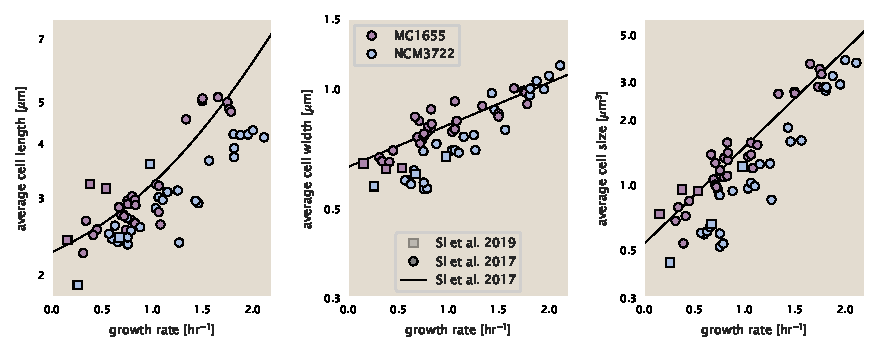
\includegraphics[width=1.0\textwidth]{SI_figs/Si_size_data_fit.pdf}
    \caption{\textbf{Summary of size measurements from Si \textit{et al.} 2017,
    2019.} Cell lengths and widths were measured from cell contours obtained from
    phase contrast images, and refer to the long and short axis respectively. (A)
    Cell lengths and (B) cell widths show the mean measurements reported (they
    report 140-300 images and 5,000-30,000 for each set of samples; which likely
    means about 1,000-5,000 measurements per mean value reported here since they
    considered about 6 conditions at a time). Fits were made to the  MG1655 strain
    data; length: 0.5 $e^{1.09 \cdot \lambda}$ + 1.76 \textmu m, width:  0.64
    $e^{0.24 \cdot \lambda}$ \textmu m. (C) Cell size, $V$, was calculated as
    cylinders with two hemispherical ends (Equation \ref{eq:cell_size}). The
    MG1655 strain data gave a best fit of 0.533 $e^{1.037 \cdot \lambda}$ \textmu m$^3$.}
  \label{fig:final_size_data_Si}
\end{figure}


\section{Estimation of Total Protein Content per Cell}
\label{sec:estimate_protein_per_cell}
In order to estimate total protein per cell for a particular growth rate, we
begin by estimating the cell size from the fit shown in Figure
\FIG{final_size_data_Si}(C) (0.533 $e^{1.037 \cdot \lambda}$ \textmu m$^3$). We
then estimate the total protein content from the total dry mass of the cell.
Here we begin by noting that  for almost the entire range of growth rates
considered here, protein, DNA, and RNA were reported to account for at least 90
\% of the dry mass (\cite{basan2015}). The authors also found that the total dry
mass concentration was roughly constant across growth conditions. Under such a
scenario, we can calculate the total dry mass concentration for protein, DNA,
and RNA, which is given by 1.1 g/ml x 30 \% x 90 \% or about $[M_P]$ = 300 fg
per fl. Multiplying this by our prediction of cell size gives the total dry mass
per cell.

However, even if dry mass concentration is relatively constant across growth
conditions, it is not obvious how protein concentration might vary due to
the substantial increase in rRNA at faster
growth rates (\cite{dai2016}). This is a well-documented result that arises from
an increase in ribosomal abundance at faster growth rates
(\cite{scott2010}). To proceed therefore rely on experimental
measurements of total DNA content per cell that also come from Basan \textit{et
al.}, and RNA to protein ratios that were measured in Dai \textit{et al.} (and
cover the entire range of growth conditions considered here). These are
reproduced in Figure \FIG{schmidt_adjustment_varying_conc}(A) and (B),
respectively.

Assuming that the protein, DNA, and RNA account for 90 \% of the total dry mass,
the protein mass can then determined by first subtracting the experimentally
measured DNA mass,  and then using the experimental estimate of the RNA to
protein ratio. The total protein per cell is will be related to the summed RNA
and protein mass by,

\begin{equation}
	M_{P} = \frac{[M_P + M_{RNA}]}{1 + (RP_{ratio})}.
\end{equation}
$(RP_{ratio}$ refers to the RNA to protein ratio as measured by Dai \textit{et
al.}. In Figure \FIG{schmidt_adjustment_varying_conc}(C) we plot the estimated
cellular concentrations for protein, DNA, and RNA from these calculations, and
in Figure \FIG{schmidt_adjustment_varying_conc}(D) we plot their total expected
mass per cell. This later quantity is the growth rate-dependent total protein
mass that was used to extimate total protein abundance across all data sets (and
summaried in \FIG{total_protein_final}(B)).


\begin{figure}
		\centering
    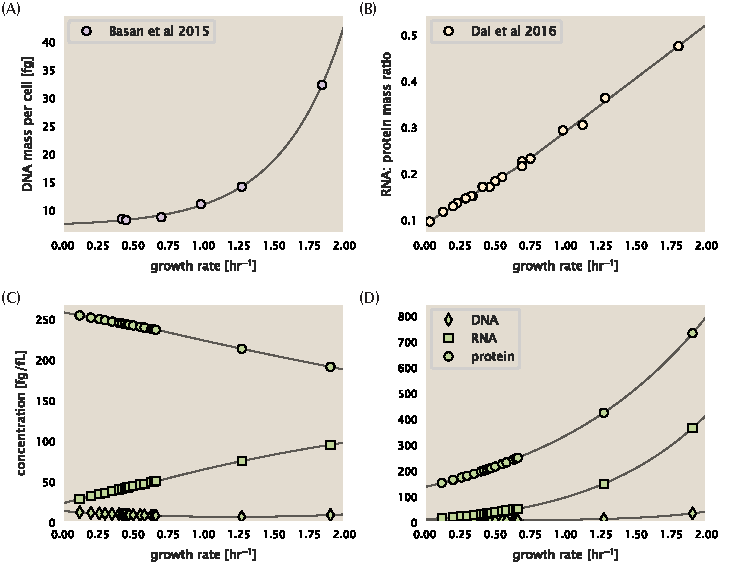
\includegraphics[width=1\textwidth]{SI_figs/schmidt_estimate_protein_RNA_DNA_corrections.pdf}
  \caption{{\bf Empirical estimate of cellular protein, DNA, and RNA as a
  function of growth rate.} (A) Measured DNA mass per cell as a function of
  growth rate, reproduced from Basan \textit{et al.} 2015. The data was fit to
  an exponential curve (DNA mass in fg per cell is given by 0.42 $e^{2.23 \cdot
  \lambda}$ + 7.2 fg per cell, where $\lambda$ is the growth rate in hr$^{-1}$).
  (B) RNA to protein measurements as a function fo growth rate. The data was for
  to two lines: for growth rates below 0.7 hr$^{-1}$, the RNA/protein ratio is
  0.18$\cdot \lambda$ + 0.093, while for growth rates faster than 0.7 hr$^{-1}$
  the RNA/protein ratio is given by 0.25$\cdot \lambda$ + 0.035. For (A) and (B)
  cells are grown under varying levels of nutrient limitation, with cells grown
  in minimal media with different carbon sources for the slowest growth
  conditions, and rich-defined media for fast growth rates. (C) Predictions of
  cellular protein, DNA, and RNA concentration.  (D) Total cellular mass
  predicted for protein, DNA, and RNA using the cell size predictions from Si
  \textit{et al.}. Symbols (diamond: DNA, square: RNA, circle: protein)
	show estimated values of mass concentration and mass per cell for the specific
	growth rates in \cite{schmidt2016}.
	 	}
  \label{fig:schmidt_adjustment_varying_conc}
\end{figure}
